%Folgende Zeile aktivieren und als SVN property "svn:keywords" auf "Id" setzen, um SVN Versionsinformationen im Dokument zu erhalten
%\svnInfo $Id: einleitung.tex 60 2012-01-26 15:56:06Z koppor $ 

\chapter{Allgemeine Verfahren}
\label{chap:k3}
	Blablalba
	\subsection {Canny-Edge-Detektor}
		Der Canny-Edge Operator is ein von John Canny 1986 entwickelter Algorithmus zur Kantendetektion. Er liefert für ein Grauwertbild möglichst alle zusammenhängenden Kanten. Der Algorithmus gliedert sich dabei im Wesentlichen in zwei Schritte:
\begin{enumerate}
	\item Kantenhervorhebung
	\item Erzeugung von Katenzügen
\end{enumerate}

Zunächst wird das Bild mit einem zweidimensionalen Gaußkern $G$ gefaltet:
{\[\large \begin{bmatrix}
1 & 2 & 1\\ 
2 & 4 & 2 \\ 
1 & 2 & 1
\end{bmatrix}\]}
Dieser sorgt dafür, dass gröbere Störungen und Rauschen beseitigt werden.
Das gefilterte Bild wird nun auf Kanten hin untersucht. Während Flächen und Segmente in Bildern meist homogene Grauwerte besitzen, stellen Kanten große Grauwertsprünge dar. Um diese Grauwertsprünge zu detektieren, verwendet man den Sobeloperator, ein Filter, der die partiellen Ableitungen eines Pixels in $x$- und $y$-Richtung liefert. \\
Die Struktur eines 1D Sobelfilters ergibt sich dabei aus der finiten Differenz (hier: Zentraldifferenz) an der Stelle $x$:
%\begin{figure}
% 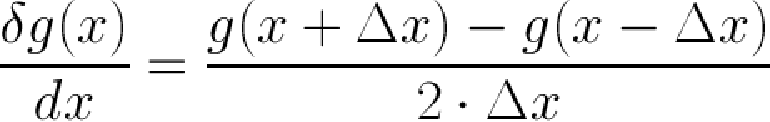
\includegraphics[width=.5\textwidth]{form1.pdf}
%\end{figure}
\begin{equation*}
\frac{\delta g(x)}{dx} = \frac{g(x + \Delta x) - g(x - \Delta x)}{2 \cdot \Delta x }
\end{equation*}
wobei $\Delta x = 1$. Damit hat der diskrete 1D Filter $S$ die Struktur
\begin{equation*}
S = \begin{bmatrix}
1 & 0 & -1
\end{bmatrix}
\end{equation*}
Erweitert auf einen zweidimensionalen Filter ergibt sich

\begin{equation*}
S(x) = \begin{bmatrix}
1 & 0 & -1\\ 
2 & 0 & -2\\ 
1 & 0 & -1
\end{bmatrix},
S(y) = \begin{bmatrix}
1 & 2 & 1\\ 
0 & 0 & 0\\ 
-1 &-2  &-1 
\end{bmatrix}
\end{equation*}

in $x$-, bzw. $y$-Richtung. \\
Die Anwendung der Filter auf das Ausgangsbild liefert die partiellen Ableitungen $G_x$ und $G_y$.
Aus diesen partiellen Ableitungen, die die Anwendung der beiden Filter liefert, lässt sich die Gradientenrichtung $d$ einer Kante berechnen:
\begin{equation*}
d(x, y) = arctan(\frac{G_y(x, y)}{G_x(x, y)})
\end{equation*}
Anschließend wird aus den partiellen Ableitungen ein Bild der absoluten Kantenstärke berechnet:
\begin{equation*}
G(x, y) = \sqrt{G_x(x, y)^2 + G_y(x, y)^2}
\end{equation*}
Im nächsten Schritt wird eine Technik names “Non-maximum suppression” angewandt, um sicherzustellen, dass Kanten nicht breiter als ein Pixel sind. Dabei werden für jedes Pixel seine 8 Nachbarn untersucht. Befindet sich in der Nachbarschaft des zu untersuchenden Pixels ein Pixel, dass einen höheren Grauwert aufweist, so wird der Grauwert des zu untersuchenden Pixels auf 0 gesetzt, es sei denn, das Pixel mit dem größeren Grauwert befindet sich entlang der Gradientenrichtung. \\ \\
Im letzten Schritt des Verfahrens werden die Pixel zu Kantenzügen zusammengefasst.
Dabei verwendet man zwei Schwellwerte $L_1 < L_2$. Zunächst wird nach einem Pixel gesucht, dessen Grauwert größer als $L_2$ ist. Dieses Pixel wird zum Startpixel des Kantenzugs erklärt. Nun wird die Kante in beiden Richtungen nach Pixel mit einem Grauwert größer $L_1$ abgesucht, welche dem Kantenzug hinzugefügt werden. Werden keine Pixel gefunden, die diese Bedingung erfüllen, bricht die Suche ab, und des wird ein neues Startpixel gesucht.Das Verfahren endet, sobald kein unmarkiertes Pixel mit einem Grauwert größer $L_2$ gefunden wird. \\ \\
Als Resultat des Verfahrens entsteht ein Bild, das eine Menge von Pixeln enthält, die idealerweise genau die Kantenpixel des Ausgangsbilds enthält.
\begin{figure}[H]
  \begin{center}
    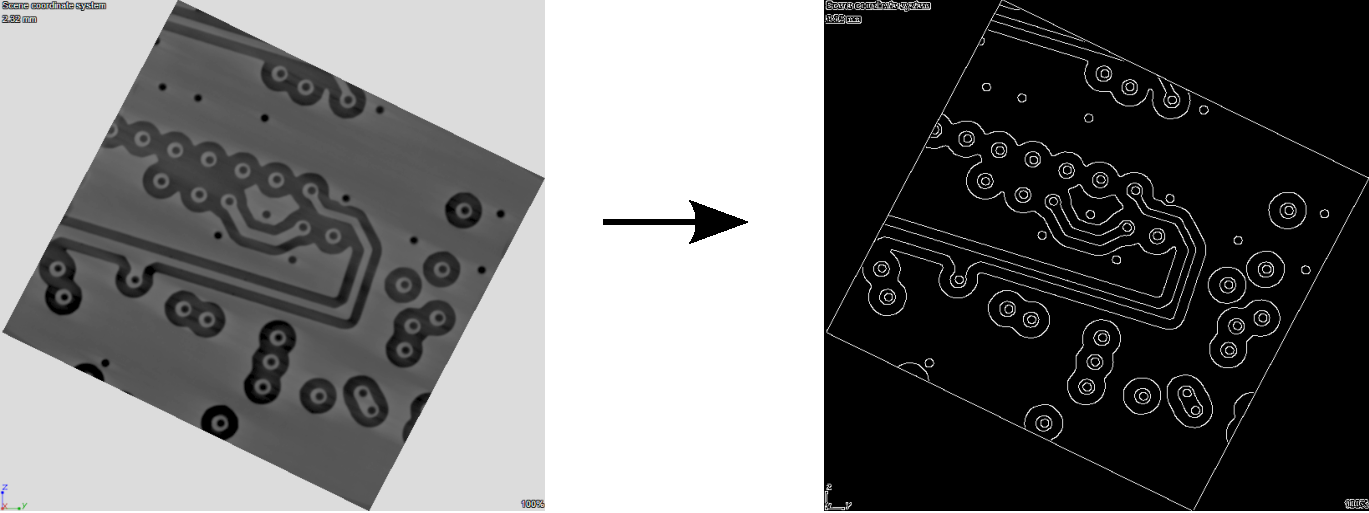
\includegraphics[width=\textwidth]{canny.pdf}
    \caption{Resultat nach der Anwendung des Canny-Edge-Detektors}
    \label{fig:canny}
  \end{center}
\end{figure}


	\subsection {Floodfill-Algorithmus}
Floodfill ist ein Algorithmus, der in multi-dimensionalen Arrays zusammenhängende Felder erkennen und färben kann. Ob Felder zusammenhängen ist abhängig davon ob sie identische Eigenschaften aufweisen. Bei zweidimensionalen Bilddaten wird dafür die Farbe der Pixel verwendet. Ausgehend von einem Startpunkt durchsucht der Algorithmus “flutartig” das Array und ändert die Suchrichtung, sobald eine Eigenschaft nicht mehr erfüllt ist. \\
Der Algorithmus betrachtet ausgehend von einem Startpunkt rekursiv alle benachbarten Felder und färbt diese gegebenenfalls. Ausgehend davon wie viele der Nachbarfelder betrachtet werden spricht man z.B. im zweidimensionalen von “fill4” (oben, unten, links, rechts) oder “fill8” (alle Nachbarn). \\ \\
Alle eingesetzten Verfahren arbeiten auf dem Resultat eines Canny-Edge-Detektors. Zusätzlich wurde bei den Verfahren, die auf einem gefärbten Bild arbeiten, eine Färbung zusammenhängender schwarzer Flächen nach folgendem Prinzip durchgeführt: \\

\begin{lstlisting}
for x in xrange(0, width, 3):   # stepsize ist 3
	for y in xrange(0, height, 3):
		fill8(img, x, y, (0,0,0), randomColor, resimg)
\end{lstlisting}

Der implementierte "fill8"-Algorithmus entspricht dem Floodfill-Algorithmus mit einer 8-Pixel Nachbarschaft, welcher im vorigen Abschnitt beschrieben wurde. Dabei wurde der Algorithmus derart modifiziert, dass zuerst in der 8er-Umgebung geprüft wurde ob ein weißer Pixel an den zu untersuchenden Pixel angrenzt und anschließend die 4er-Umgebung auf den Stack gelegt wurde, falls die Prüfung negativ ausgefallen ist. Durch diesen Trick wird verhindert, dass der Algorithmus durch kleinere Lücken (bis 2 Pixel) des Canny-Bildes, welche aufgrund von von fehlerhafter Erkennung entstehen, nicht hindurch läuft.

\begin{figure}[H]
  \begin{center}
    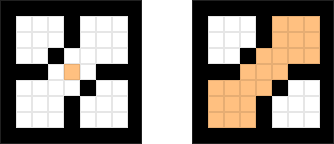
\includegraphics[width=0.6\textwidth]{floodfill.png}
    \caption{fill4 färbt ausgehend vom Mittelpunkt die zentrale, weiße Fläche.}
    \label{fig:floodfill}
  \end{center}
\end{figure}

	\subsection {Houghtransformation}
Die Houghtransformation baut auf der Kantendetektion auf: Sie sucht Formen, die von Kantenpunkten gebildet werden.
Die Houghtransformation ist sehr allgemein verwendbar; Formen können im einfachsten Fall Geraden oder Kreise sein, es können aber auch Ellipsen und andere geometrische Figuren detektiert werden, es handelt sich bei der Houghtransformation also um eine \textbf{modellbasiertes} Verfahren.
Mit der verallgemeinerten Houghtransformation können sogar beliebige Formen gefunden werden.
Die Houghtransformation benutzt ein einfaches Grundprinzip: Man untersucht alle Kantenpunkte auf Hinweise auf eine gegebene Form, die man detektieren möchte. Diese Hinweise werden in einem Akkumulatorraum (Parameterraum) gespeichert. Nachdem alle Kantenpunkte untersucht wurden, wertet man die gesammelten Hinweise im Akkumulatorraum aus.
Die Untersuchung der Kantenpunkte und die Dimension des Akkumulatorraums hängen dabei von der Form ab, die man detektieren will.
		\subsubsection{Houghtransformation zur Erkennung von Geraden}
			Wendet man auf ein Bild die üblichen Katenfilter an (Sobel-Operator, Canny-Edge-Detektor) zeigt sich, dass diese Verfahren zwar eine Menge von Punkten liefern, die auf Kanten, bzw. Geraden liegen, die Zusammenfassung dieser Punkte zu echten Kanten allerdings fehlt. Hier setzt die Houghtransformation an, indem es ein zusammenhängendes Geradenstück auf einen Punkt im Akkumulatorraum abbildet. \\
Eine Gerade, beschrieben durch die Gleichung $y = mx + b$ würde also auf einen Punkt im zweidimensionalen Akkumulatorraum, der durch $m$ und $b$ aufgespannt wird, abgebildet werden. Dies hat jedoch den Nachteil, dass senkrechte Geraden eine unendliche Steigung haben, sodass diese nicht mehr korrekt in den Akkumulatorraum abgebildet werden können. \\
Stattdessen verwendet man die Hessesche Normalform zur Darstellung der Geraden:
\begin{equation*}
r = x \cdot cos (\theta _0) + y \cdot sin (\theta _0) , \theta _0 \in [0, \pi [
\end{equation*}

Der zugehörige Akkumulatorraum $A$ wird damit von $\theta$ und $r$ aufgespannt.

Zunächst wird das Ausgangsbild mit einem Kantendektektor gefiltert (z.B. mit dem Sobel-Filter), woraus sich eine Matrix der Gradientenstärke $G(x, y)$ und der Gradientenrichtung $\theta (x, y)$ berechnen lässt (siehe Canny-Edge-Detektor). \\
Auf $G(x, y)$ wird nun ein Schwellwert $G^*$ angewandt, um die $N$ Pixel zu erhalten, die nicht durch kleinere Grauwertschwankungen im Ausgangsbild verursacht wurden.  Man erhält die Menge
\begin{equation*}
M = \left \{ (x_i, y_i, \theta _i) | G(x_i, y_i) \geq G^*, \theta _i=\theta (x, y), i = 1...N \right \}
\end{equation*}

aus Kantenpunkten und -richtungen. \\
Im nächsten Schritt "Votiert" jedes Element $(x_i, y_i, \theta_i) \in M$ für einen Punkt $(\theta_i, r)$ im Akkumulatorraum, indem der Wert um 1 erhöht wird:
\begin{itemize}
\item $\forall (x_i, y_i \theta_i) \in M:$
	\begin{enumerate}
		\item $r = x_i \cdot cos(\theta_i) + y \cdot sin(\theta_i)$
		\item {Erhoehe $(\theta_i, r_i)$ um 1}
	\end{enumerate}
\end{itemize}

\begin{figure}[H]
  \begin{center}
    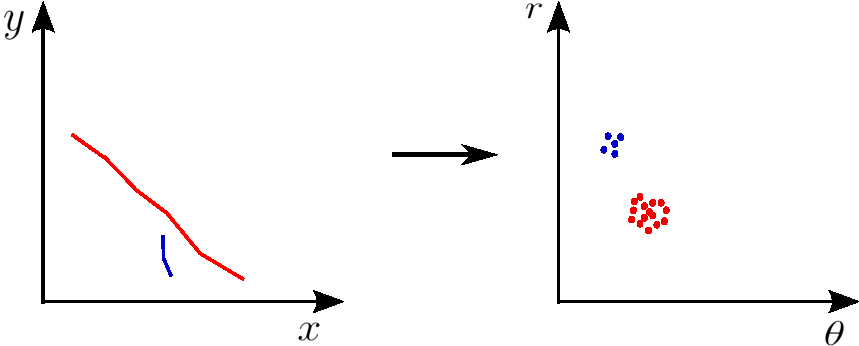
\includegraphics[width=\textwidth]{akku.pdf}
    \caption{Abbildung der Geraden in den Akkumulatorraum}
    \label{fig:akku}
  \end{center}
\end{figure}

Alle Punkte, die auf einer Geraden liegen, votieren somit für den gleichen Punkt in $A$. \\ 
Allerdings werden Punkte einer Geraden aufgrund von Ungenauigkeiten nicht exakt für den selben Punkt $A(\theta_i, r_i)$ votieren, sondern einen Cluster bilden. Daher genügt es nicht, im Akkumulatorraum nach großen Werten zu suchen, sondern es ist zusätzlich eine Clusteranalyse notwendig, um alle Punkte auf der Geraden zu ''erwischen".
\begin{figure}[H]
  \begin{center}
    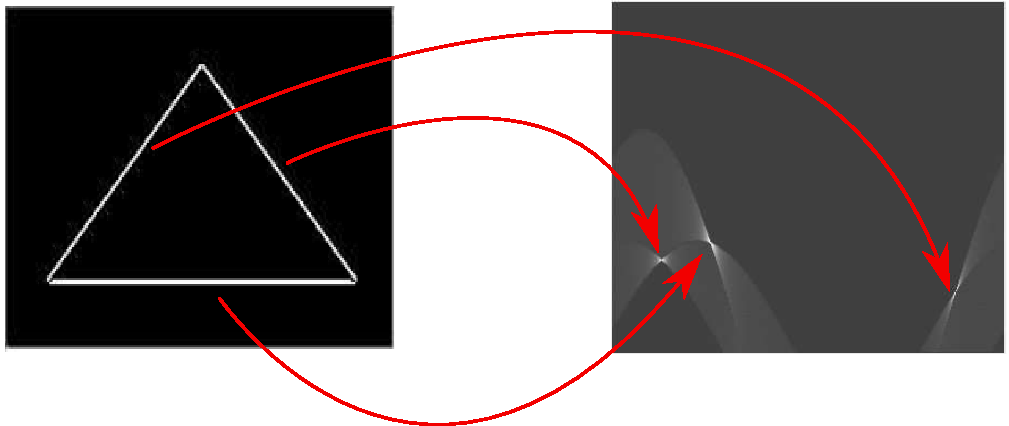
\includegraphics[width=\textwidth]{akku_projection.pdf}
    \caption{Dreiecksgeraden werden in den Akkumulatorraum projeziert}
    \label{fig:akku_projection}
  \end{center}
\end{figure}
 

			
		\subsubsection{Houghtransformation Erkennung von Kreisen}

	

%\vspace{-3cm}
%\vspace{2cm}



